\chapter{Signal systematics}\label{ch:signal_systematics}
There are several factors that contribute to the systematic uncertainty on the signal yields, which must be accounted for when checking for significant excesses in the signal region or when setting limits on signal production.
The dominant sources of systematic error are the large-R jet mass scale (JMS), the small-R b-tagging uncertainty, the Monte Carlo statistical uncertainty, and the modelling uncertainty, which includes uncertainty on parton distribution functions (PDFs), QCD scale uncertainty, and initial state radiation (ISR) modelling uncertainty.
The size of the contribution from each source of uncertainty depends on the signal point being evaluated.
To evaluate the size of a systematic uncertainty from a given source, a nuisance parameter is varied up and down, and the variation in the signal yield as compared to the nominal value is taken as the size of the uncertainy.
When a systematic contains multiple components, those components are treated as uncorrelated, and their contributions are combined in quadrature.

For example, to evaluate the contribution to the signal efficiency uncertainty from PDF, QCD scale, $\alpha_s$ and ISR modelling uncertainties, truth-level signal simulation samples are created where different parameters are varied in the generation.
For PDF uncertainties, the internal event weights in the PDF set are varied up and down during the generation.
For the QCD scale and $\alpha_{s}$ uncertainties, the value of these parameters are varied up and down during the generation.
For ISR uncertainties, the value of the matching scale, $q_{\textrm{cut}}$ is varied up and down during the generation.
Figures~\ref{fig:systematics_njet,fig:systematics_nbjet,fig:systematics_deta,fig:systematics_mj} show the nominal and systematically-shifted distributions of four observables that contribute to the signal region definition for four representative signal points.
The nuisance parameters varied in these plots are the event internal weights of the PDF set, the QCD scale, and $\alpha_{S}$.
The PDF and QCD scale contributions to the uncertainty are highest at low gluino mass, reaching a maximum of $25\%$ at$m_{\tilde{g}}=1.0~TeV$, the lowest gluino mass studied.
For higher masses, these uncertainties drop to only a few percent.
For reconstruction-level uncertainties such as b-tagging efficiency, the nominal signal samples are used, and the detector simulation is run with different nuisance parameters separately shifted up or down.

\begin{figure}[!ht]
    \centering
    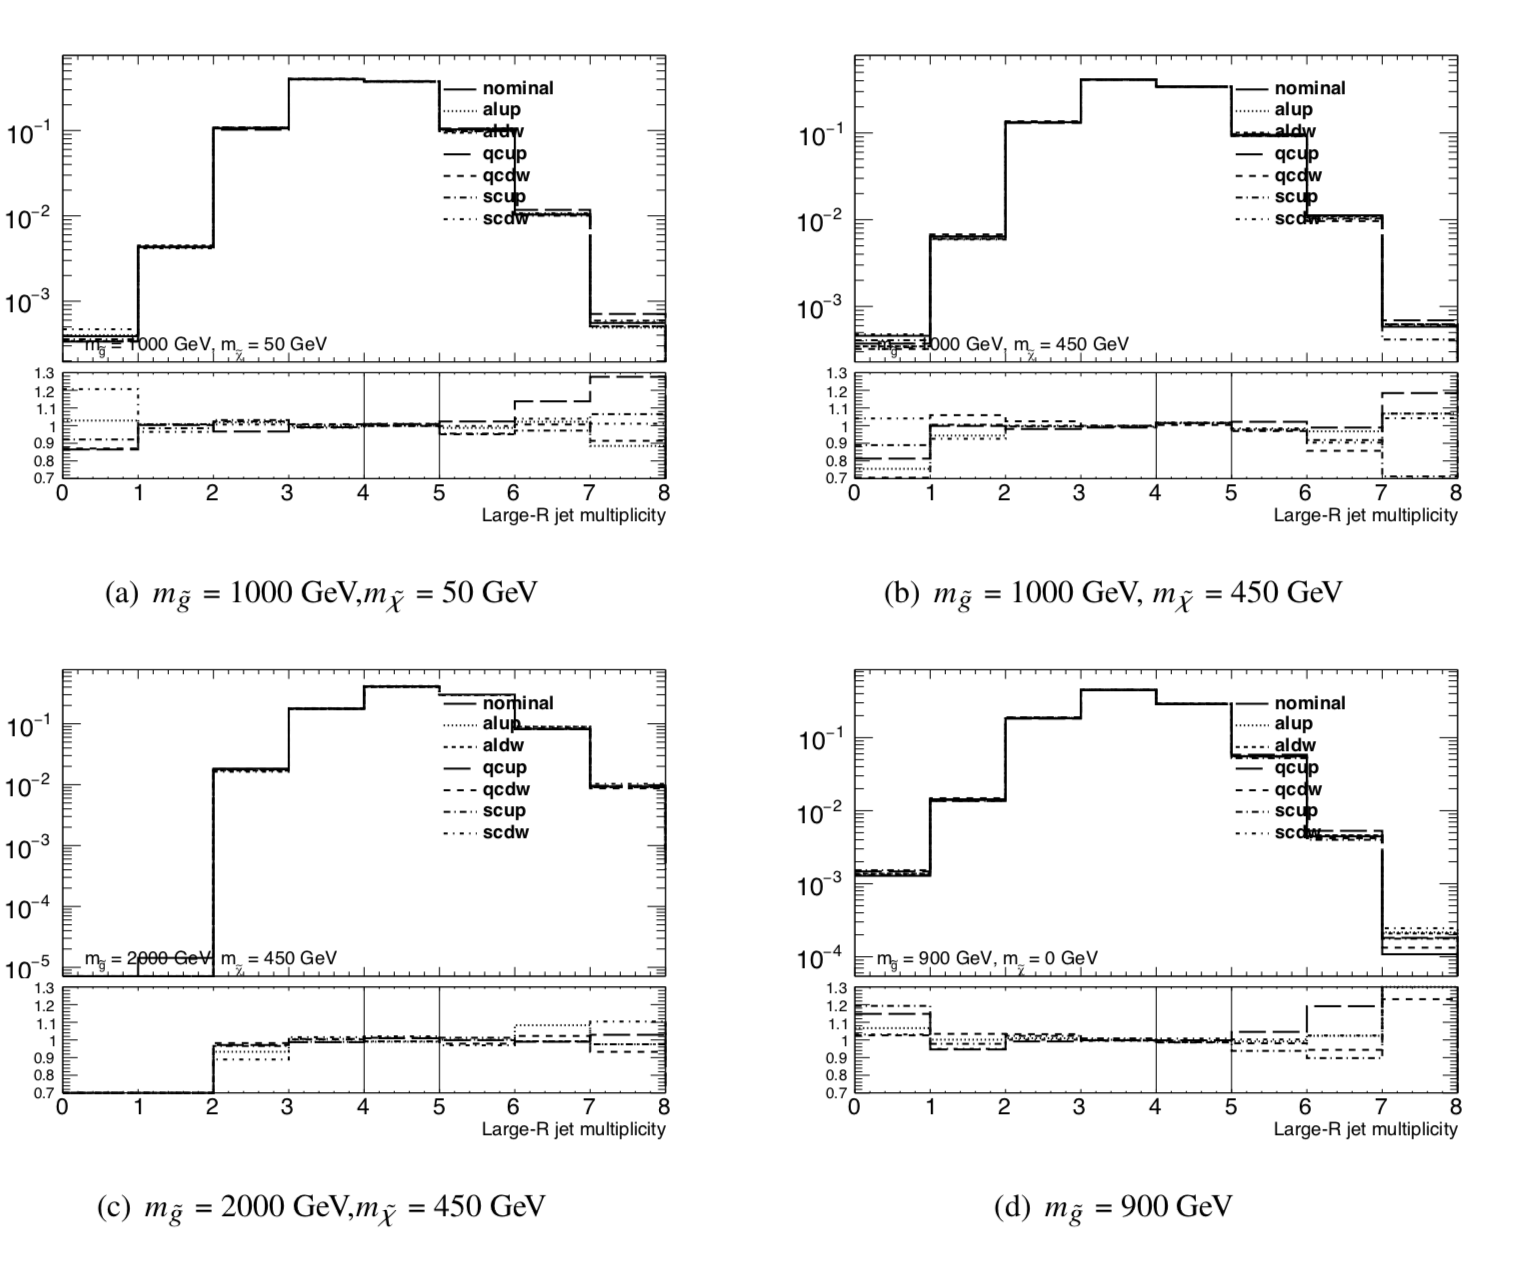
\includegraphics[width=0.9\textwidth]{systematics_njet_variation}
    \caption{Nominal and systematically-shifted $N_{jet}$ distributions for four signal points, showing the shifted distributions for internal generator event weights, QCD scale, and $\alpha_{s}$.}
    \label{fig:systematics_njet}
\end{figure}

\begin{figure}[!ht]
    \centering
    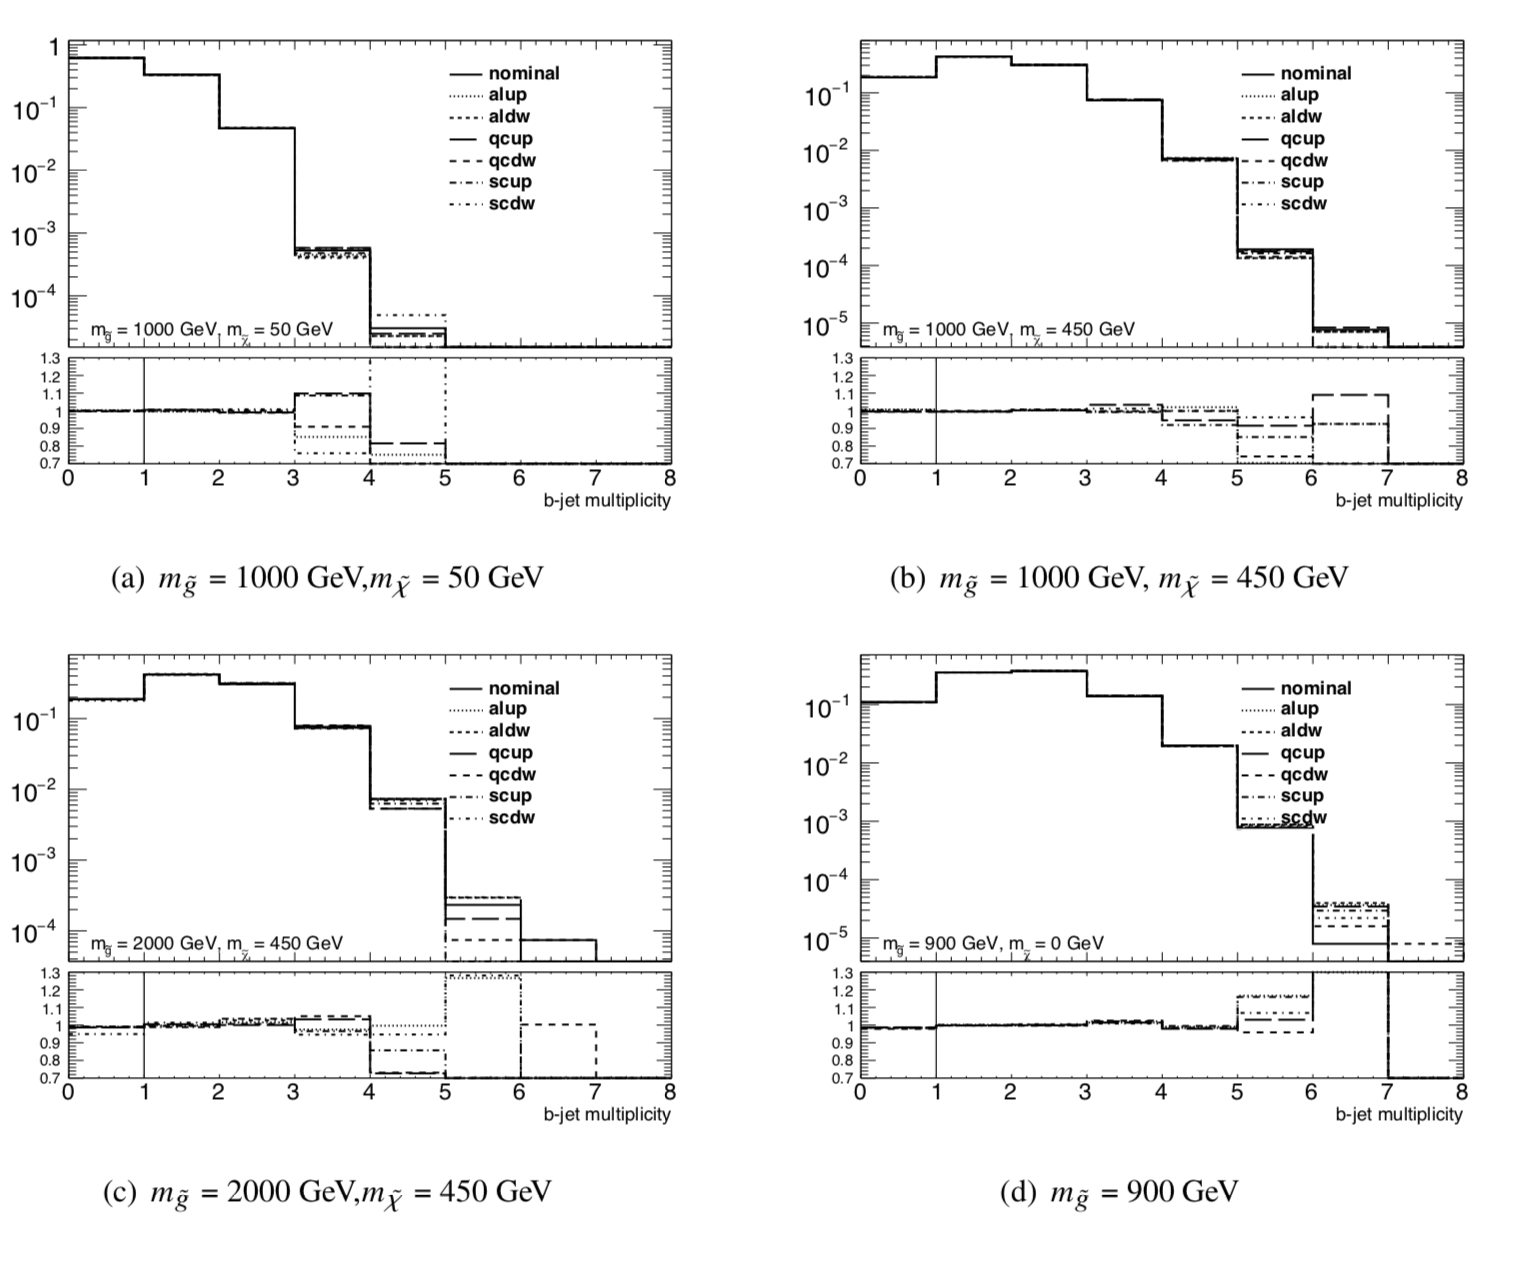
\includegraphics[width=0.9\textwidth]{systematics_nbjet_variation}
    \caption{Nominal and systematically-shifted $N_{b-jet}$ distributions for four signal points, showing the shifted distributions for internal generator event weights, QCD scale, and $\alpha_{s}$.}
    \label{fig:systematics_nbjet}
\end{figure}

\begin{figure}[!ht]
    \centering
    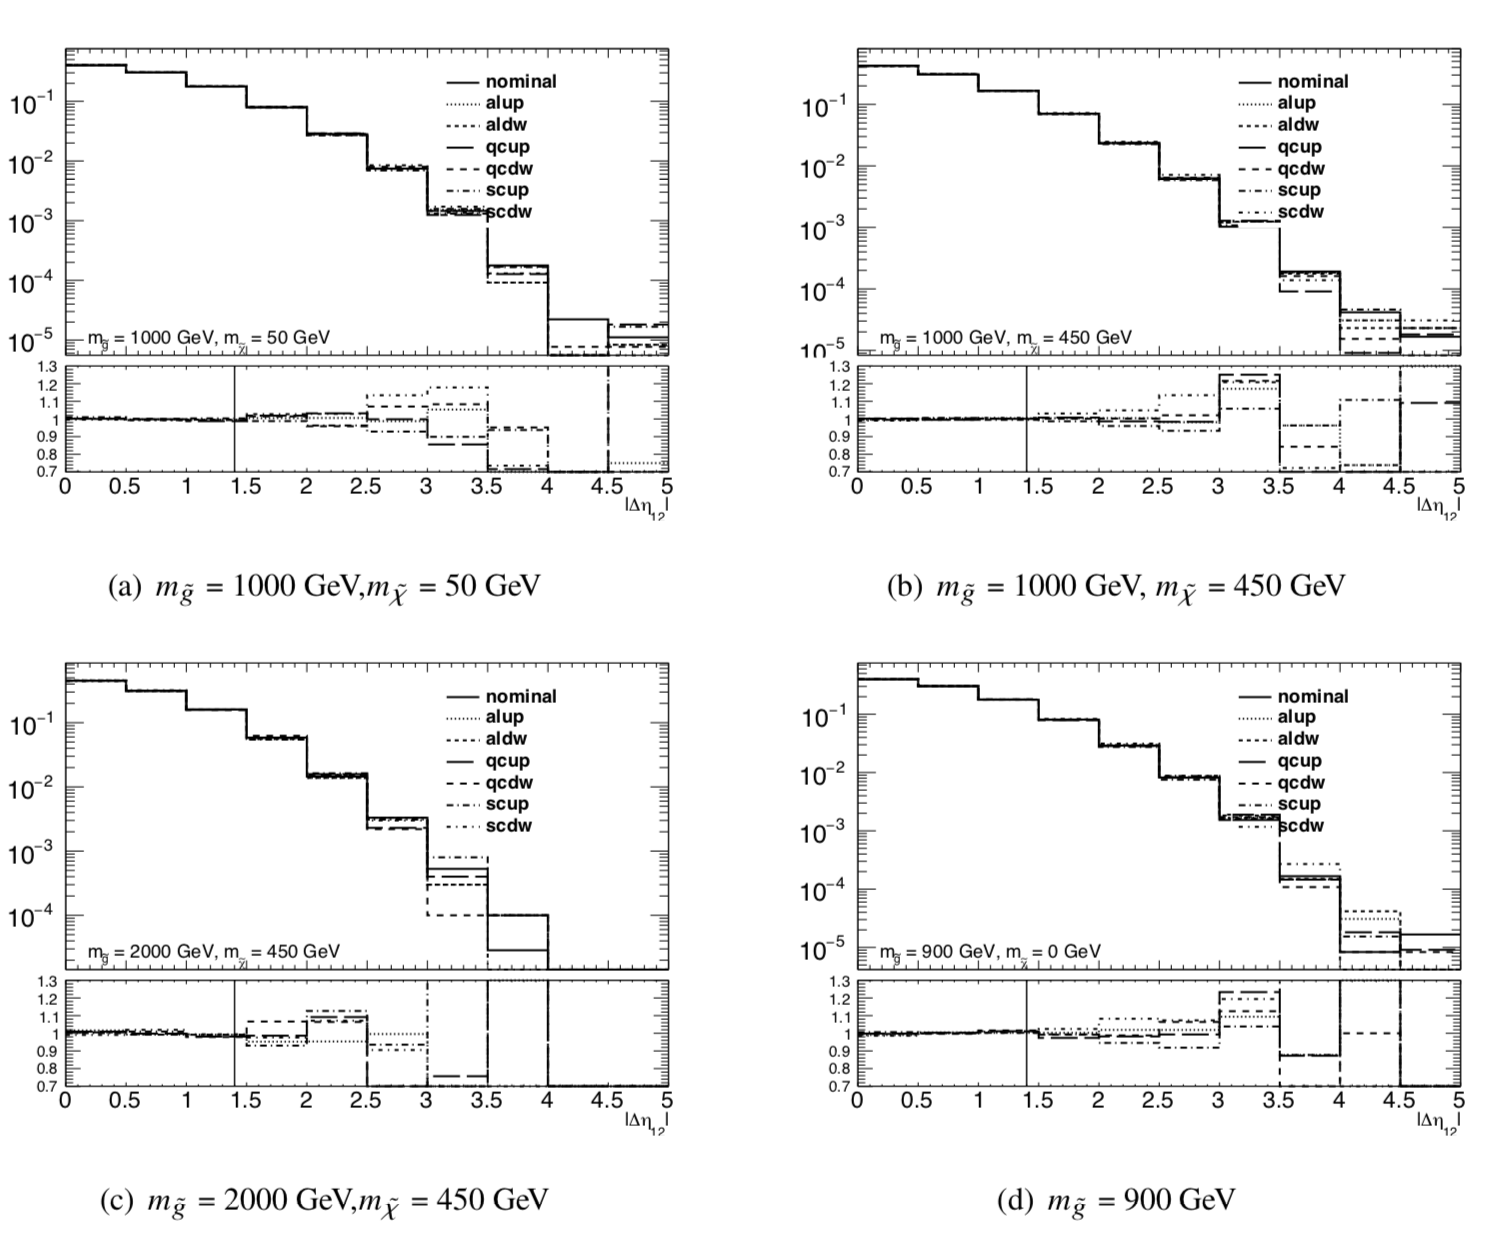
\includegraphics[width=0.9\textwidth]{systematics_deta_variation}
    \caption{Nominal and systematically-shifted $|\Delta\eta_{1,2}|$ distributions for four signal points, showing the shifted distributions for internal generator event weights, QCD scale, and $\alpha_{s}$.}
    \label{fig:systematics_deta}
\end{figure}

\begin{figure}[!ht]
    \centering
    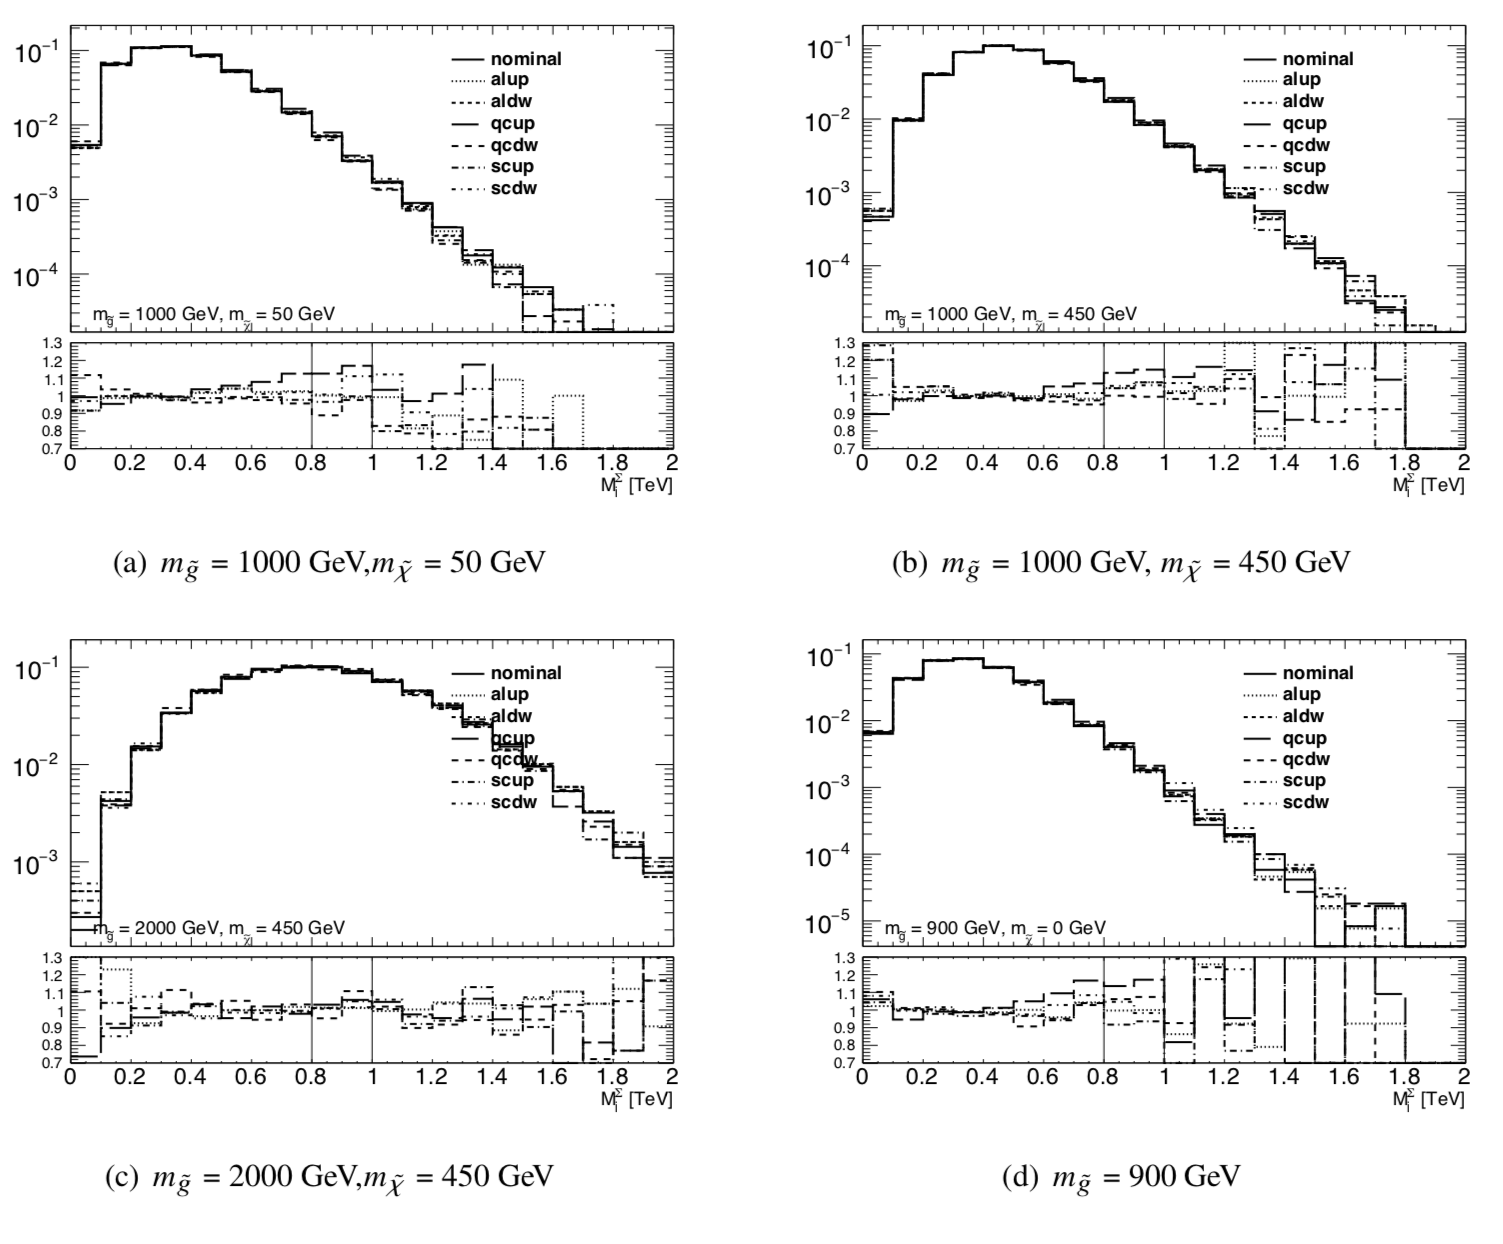
\includegraphics[width=0.9\textwidth]{systematics_mj_variation}
    \caption{Nominal and systematically-shifted $M_{J}^{\Sigma}$ distributions for four signal points, showing the shifted distributions for internal generator event weights, QCD scale, and $\alpha_{s}$.}
    \label{fig:systematics_mj}
\end{figure}

For the large-$R$ JMS, there are four components, called the baseline, modeling, statistical, and tracking components.
These components are derived from the $R_{trk}$ method~\cite{jet-substructure-perf}.
The JMS uncertainty is largest for $m_{\tilde{g}}=1.0~TeV$, at $\approx 24\%$, and drops to $\approx 8\%$ for signal points with $m_{\tilde{g}}=1.8~TeV$.
It is generally dominated by the tracking uncertainty, followed by the baseline uncertainty.
The b-tagging uncertainty is evaluated by varying a set of 25 nuisance parameters.
The result is an uncertainty on the signal efficiency of between $15\%$ and $25\%$.
This uncertainty is only applied to the b-tag signal regions.
The luminosity uncertainty is 3.2\%, and other uncertainties such as small-$R$ jet energy scale (JES), small-$R$ jet energy resolution (JER), and pileup are found to be negligible.
Table\ref{tbl:systematics_summary} gives a summary of the sources of systematic uncertainty, the number of nuisance parameters for each source, and the approximate range of uncertainty size for each source.
Because the size of the uncertainty depends strongly on the particular signal point, these are only approximate ranges, except in the case of luminosity, where the uncertainty is the same regardless of signal point.
The JMS uncertainty is highest for the lowest-mass signal points, and decreases with gluino mass.
The $b$-tagging efficiency uncertainty is only relevant for signal regions that include a $b$-tag requirement.
\begin{table}[!ht]\centering
\begin{tabular}{lll}
    \toprule
    source                              & number of nuisance parameters & size of uncertainty    \\ \midrule
    b-tagging efficiency                & 25                            & $15\%-25\%$            \\ \midrule
    \multirow[t]{4}{*}{Large-$R$ JMS}   & \multirow[t]{4}{*}{4}         & baseline: $4\%-10\%$   \\
                                        &                               & modeling: $3\%-6\%$    \\
                                        &                               & statistical: $5\%-8\%$ \\
                                        &                               & tracking: $9\%-17\%$   \\ \midrule
    PDF, QCD Scale, and $\alpha_{s}$    & 3                             & $5\%-25\%$             \\ \midrule
    luminosity                          & 1                             & $3.2\%$                \\ \bottomrule
\end{tabular}
\caption{Summary of contributions to systematic uncertainties on the signal yield from various sources, including the number of nuisance parameters and approximate range of uncertainty size for each.}
\label{tbl:systematics_summary}
\end{table}


